\chapter{Pengendapan dan Kelarutan}\label{ch:b1:precipitation}

Setetes perak nitrat jatuh ke dalam air keran dan muncullah awan putih:
perak klorida, yang terbentuk dari beberapa miligram ion klorida yang
terdapat dalam setiap liter. Air yang merembes melalui batu kapur
membawa pergi kalsium karbonat dan mengendapkannya kembali, sepersekian
milimeter setahun, sebagai stalaktit sebuah gua. Batu ginjal pun sebuah
endapan. Masing-masing merupakan kesetimbangan antara sebuah padatan dan
ion-ionnya dalam larutan, dan satu tetapan, \omterm{def:b1:precipitation:solubility-product}{hasil kali kelarutan},
menyatakan apakah padatan itu terbentuk, berapa banyak yang larut, dan
bagaimana \omterm{def:b1:precipitation:solubility}{kelarutannya} berubah jika ditambahkan ion lain atau jika pH
diubah. Dengan tetapan itu seorang ahli kimia dapat memisahkan ion-ion
satu dari yang lain dengan mengendapkannya secara bergiliran --- dasar
pengolahan air tambang yang menutup bab ini.

\begin{recall}
Jilid sekolah (kelas 6 dan 12) mengukur \omterm{def:b1:precipitation:solubility}{kelarutan} dalam gram per liter
dan mengenali ion-ion dari endapan yang dihasilkannya. Tetapan
kesetimbangan, \omterm{def:b1:extent-q-and-k:quotient}{kuosien reaksi} $Q$, dan \omterm{def:b1:extent-q-and-k:activity}{aktivitas} (1 untuk padatan murni
atau pelarut, $c/c^\circ$ untuk zat terlarut) disusun pada
\cref{ch:b1:extent-q-and-k}: reaksi berlangsung maju selama $Q < K$.
Metode \omterm{def:b1:predominant-reaction:predominant-reaction}{reaksi predominan} dan skala $\mathrm{p}K_a$ berasal dari
\cref{ch:b1:predominant-reaction}; $c^\circ = \qty{1}{mol/L}$ tidak
dituliskan dalam kuosien.
\end{recall}

\begin{omfigure}
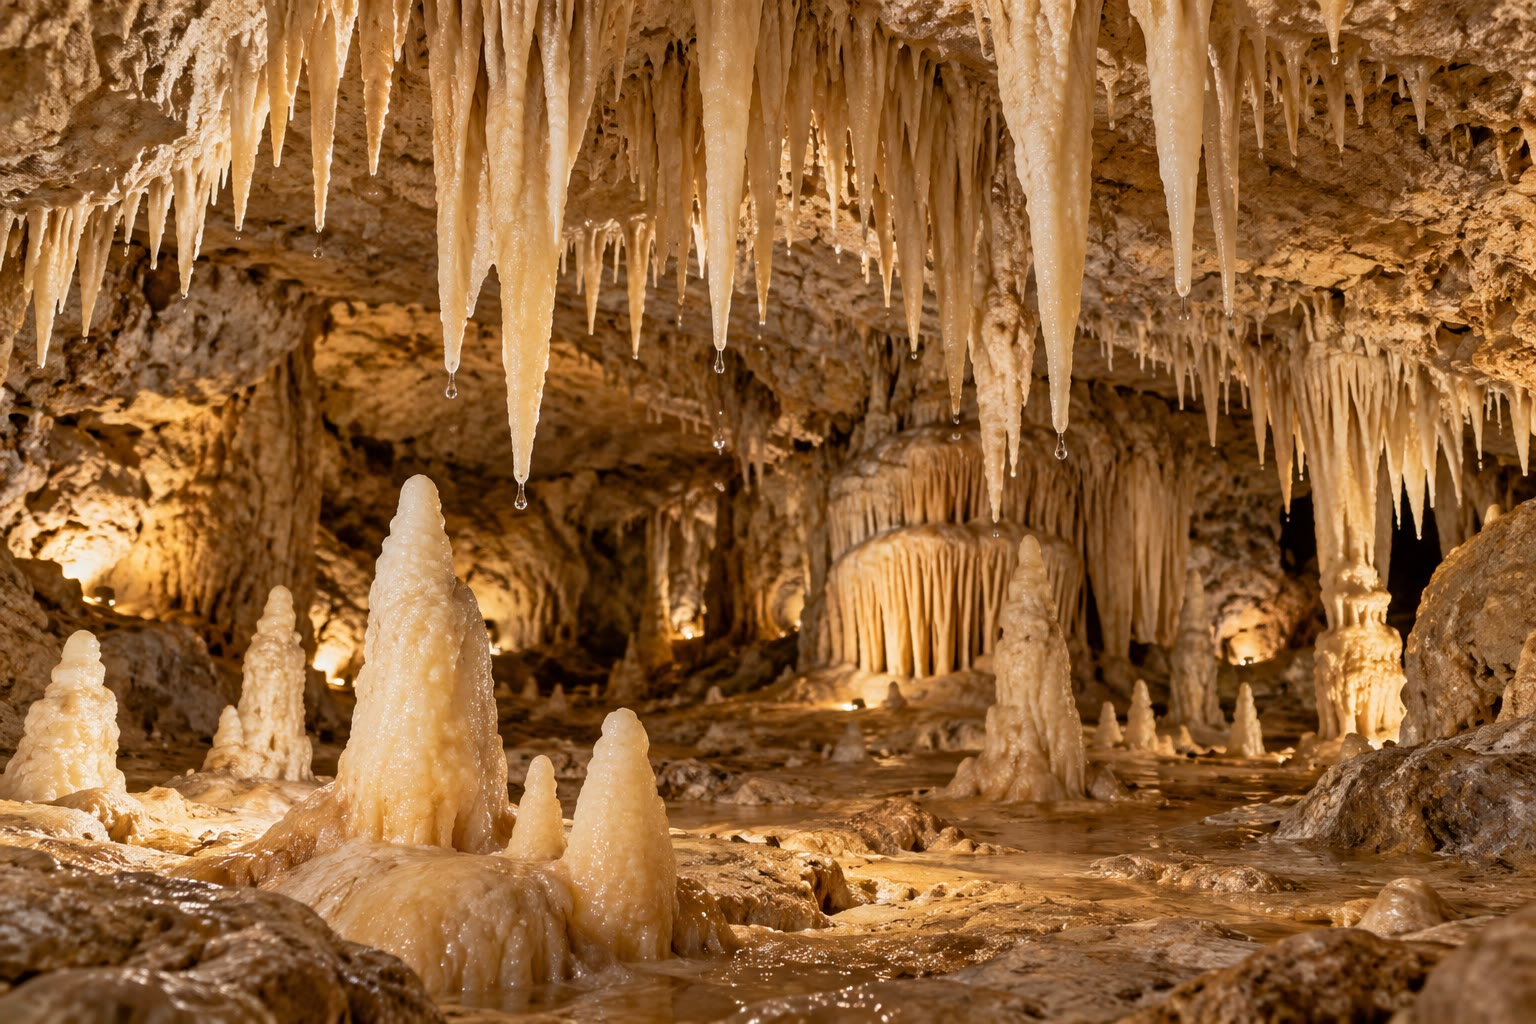
\includegraphics[width=0.62\linewidth]{images/book2/ai/b1-11-cave.jpg}

{\small Stalaktit dan stalagmit di dalam gua batu kapur. Air yang kaya
karbon dioksida melarutkan kalsium karbonat di dalam tanah di atasnya; di
dalam gua air itu kehilangan sebagian karbon dioksidanya dan karbonatnya
mengendap kembali (\cref{exo:b1:precipitation:10}).}
\end{omfigure}

\section{Hasil kali kelarutan}\label{sec:b1:precipitation:product}

Sebuah \omterm{def:b1:crystals-metals:crystal}{kristal} perak klorida yang dijatuhkan ke dalam air melepaskan ion
ke larutan, dan larutan itu mengembalikan sebagian ion ke \omterm{def:b1:crystals-metals:crystal}{kristal}. Jika
kedua laju itu sama, larutannya \emph{jenuh}: komposisinya tidak lagi
berubah, walaupun ion-ion terus berpindah ke kedua arah (gambar di
bawah).

\begin{definition}[Hasil kali kelarutan]\label{def:b1:precipitation:solubility-product}
\emph{Hasil kali kelarutan}\index{hasil kali kelarutan} $K_s$ sebuah
padatan ion $\mathrm{M}_a\mathrm{X}_b$ adalah tetapan kesetimbangan
pelarutannya menjadi ion-ionnya,
\[
  \mathrm{M}_a\mathrm{X}_b\mathrm{(s)} \rightleftharpoons a\,\mathrm{M}^{m+}
  + b\,\mathrm{X}^{x-}, \qquad
  K_s = [\mathrm{M}^{m+}]_{\mathrm{eq}}^{\,a}\,[\mathrm{X}^{x-}]_{\mathrm{eq}}^{\,b},
  \qquad \mathrm{p}K_s = -\log K_s ,
\]
karena \omterm{def:b1:extent-q-and-k:activity}{aktivitas} padatannya 1. Seperti setiap tetapan kesetimbangan,
hasil kali \omterm{def:b1:precipitation:solubility}{kelarutan} hanya bergantung pada suhu.
\end{definition}

Untuk perak klorida, \ce{AgCl(s) <=> Ag+ + Cl-} dan $K_s =
[\ce{Ag+}][\ce{Cl-}] = 10^{-9.75}$; untuk kalsium fluorida, \ce{CaF2(s) <=>
Ca^2+ + 2F-} dan $K_s = [\ce{Ca^2+}][\ce{F-}]^2 = 10^{-9.84}$; untuk
besi(III) hidroksida, $K_s = [\ce{Fe^3+}][\ce{OH-}]^3 = 10^{-38.55}$.
Tabel di bawah memuat nilai-nilai yang dipakai dalam jilid ini.
Nilai-nilai itu dihitung, seperti $\mathrm{p}K_a$ pada
\cref{ch:b1:predominant-reaction}, dari energi Gibbs pembentukan standar
dalam tabel: $\mathrm{p}K_s = \Delta_r G^\circ/(RT\ln 10)$, sebuah hubungan
yang diturunkan dalam jilid Tahun~2.

\begin{omfigure}
\begin{tikzpicture}[font=\small, >={Stealth}]
  % the crystal: alternating Ag+ (small, grey) and Cl- (large, green)
  \foreach \i in {0,1,2,3,4,5}
    \foreach \j in {0,1,2} {
      \pgfmathtruncatemacro{\pp}{mod(\i+\j,2)}
      \ifnum\pp=0
        \shade[ball color=green!55!black!60] (\i*0.62,\j*0.62) circle (0.29);
      \else
        \shade[ball color=gray!35] (\i*0.62,\j*0.62) circle (0.17);
      \fi }
  \draw[thick, gray] (-0.45,-0.45) rectangle (3.55,1.75);
  \node[below] at (1.55,-0.45) {\ce{AgCl(s)}};
  % ions in solution
  \shade[ball color=gray!35] (1.2,3.0) circle (0.17);
  \node[right] at (1.4,3.0) {\ce{Ag+}};
  \shade[ball color=green!55!black!60] (2.6,2.7) circle (0.29);
  \node[right] at (2.9,2.7) {\ce{Cl-}};
  \shade[ball color=gray!35] (4.4,1.4) circle (0.17);
  \shade[ball color=green!55!black!60] (5.1,2.6) circle (0.29);
  \shade[ball color=gray!35] (-1.0,2.4) circle (0.17);
  \shade[ball color=green!55!black!60] (-0.6,3.3) circle (0.29);
  % arrows: dissolution and precipitation
  \draw[->, thick, omDef] (1.24,1.6) to[bend left=20] node[left, pos=0.6] {pelarutan} (1.15,2.78);
  \draw[->, thick, omProp] (2.55,2.38) to[bend left=20] node[right, pos=0.45] {pengendapan} (2.45,1.55);
  % the water line
  \draw[blue!50, thick] (-1.6,3.8) -- (5.9,3.8);
  \node[blue!60!black, anchor=east] at (5.9,4.05) {larutan jenuh};
\end{tikzpicture}

{\small Sebuah \omterm{def:b1:crystals-metals:crystal}{kristal} perak klorida di dalam larutan jenuhnya. Ion-ion
meninggalkan permukaan (pelarutan) dan ion-ion lain ditangkap
(pengendapan) dengan laju yang sama, sehingga $[\ce{Ag+}][\ce{Cl-}]$ tetap
sama dengan $K_s$. Ion perak digambar lebih kecil daripada ion klorida,
sesuai kenyataannya.}
\end{omfigure}

\begin{omfigure}
\begin{tabular}{lc@{\qquad}lc}
\hline
padatan & $\mathrm{p}K_s$ & padatan & $\mathrm{p}K_s$ \\
\hline
\ce{AgCl} & 9.75 & \ce{Ca(OH)2} & 5.33 \\
\ce{AgBr} & 12.27 & \ce{Mg(OH)2} & 11.25 \\
\ce{AgI} & 16.07 & \ce{Fe(OH)2} & 16.31 \\
\ce{Ag2CrO4} & 11.95 & \ce{Zn(OH)2} & 16.38 \\
\ce{BaSO4} & 9.97 & \ce{Fe(OH)3} & 38.55 \\
\ce{CaCO3} (kalsit) & 8.30 & \ce{Al(OH)3} (gibsit) & 34.75 \\
\ce{CaF2} & 9.84 & & \\
\hline
\end{tabular}

\smallskip
{\small \omterm{def:b1:precipitation:solubility-product}{Hasil kali kelarutan} pada \qty{25}{\celsius}, yang dihitung dari
energi Gibbs pembentukan standar padatan-padatan dan ion-ion berair.
Tetapan pembentukan yang dipakai dalam bab ini (\cref{sec:b1:precipitation:amphoteric}):
$\log\beta_4 = 14.45$ untuk \ce{Zn(OH)4^2-}, 33.52 untuk \ce{Al(OH)4-},
dan $\log\beta_1 = 11.82$ untuk \ce{FeOH^2+}.}
% ledger: dfg:AgCl_cr, dfg:AgBr_cr, dfg:AgI_cr, dfg:Ag2CrO4_cr, dfg:Ag+_ao, dfg:Cl-_ao, dfg:Br-_ao, dfg:I-_ao, dfg:CrO42-_ao (computed in figdata/bachelor-1/aqueous-constants.py)
% ledger: dfg:BaSO4_cr, dfg:Ba2+_ao, dfg:SO42-_ao, dfg:CaCO3_cr, dfg:CO32-_ao, dfg:CaF2_cr, dfg:Ca2+_ao, dfg:F-_ao (computed, same script)
% ledger: dfg:Ca_OH2_cr, dfg:Mg_OH2_cr, dfg:Mg2+_ao, dfg:Fe_OH2_cr, dfg:Fe2+_ao, dfg:Zn_OH2_cr, dfg:Zn2+_ao, dfg:Fe_OH3_cr, dfg:Fe3+_ao, dfg:Al2O3.3H2O_cr, dfg:Al3+_ao, dfg:OH-_ao (computed, same script)
% ledger: dfg:Zn_OH42-_ao, dfg:Al_OH4-_ao, dfg:FeOH2+_ao (formation constants, same script)
\end{omfigure}

\begin{proposition}[Syarat pengendapan]\label{prop:b1:precipitation:precipitation-condition}
Misalkan sebuah larutan mengandung ion-ion padatan $\mathrm{M}_a\mathrm{X}_b$,
dengan \omterm{def:b1:extent-q-and-k:quotient}{kuosien reaksi} $Q_s = [\mathrm{M}^{m+}]^a[\mathrm{X}^{x-}]^b$ untuk
pelarutannya.
\begin{itemize}
  \item Jika $Q_s < K_s$, padatan itu tidak dapat ada pada kesetimbangan:
        larutannya tidak jenuh dan padatan apa pun yang ditambahkan
        melarut, sepenuhnya jika jumlahnya tidak terlalu banyak.
  \item Jika $Q_s > K_s$, padatan itu mengendap sampai $Q_s = K_s$.
  \item Padatan dan larutan hanya berdampingan dalam kesetimbangan jika
        $Q_s = K_s$.
\end{itemize}
\end{proposition}

\begin{proof}
Menurut \cref{ch:b1:extent-q-and-k}, pelarutan berlangsung maju selama
$Q_s < K_s$ dan mundur (pengendapan) selama $Q_s > K_s$. Selama pelarutan
berlangsung maju, $Q_s$ bertambah. Jika padatannya habis sebelum $Q_s$
mencapai $K_s$, evolusinya berhenti tanpa sisa padatan: reaksi yang
melibatkan \omterm{def:b1:extent-q-and-k:system}{fase} terkondensasi murni dapat berhenti sebelum kesetimbangan
karena jumlah \omterm{def:b1:extent-q-and-k:system}{fase} itu tidak dapat menjadi negatif. Jika $Q_s > K_s$,
pengendapan menurunkan kedua konsentrasi ion dan $Q_s$ berkurang sampai
sama dengan $K_s$, yang selalu mungkin, karena ion-ionnya ada.
\end{proof}

Butir terakhir inilah yang membedakan padatan dari spesies terlarut.
Spesies asam--basa ada pada setiap pH, sekecil apa pun jumlahnya; padatan
ada atau tidak ada. Itulah sebabnya diagramnya akan berupa diagram
\emph{keberadaan}, bukan \omterm{def:b1:predominant-reaction:predominance}{diagram predominansi}
(\cref{sec:b1:precipitation:domains}).

\begin{example}[Mencampur dua larutan]\label{ex:b1:precipitation:mixing}
\qty{10.0}{mL} perak nitrat \qty{2.0e-4}{mol/L} dicampur dengan
\qty{10.0}{mL} natrium klorida \qty{2.0e-4}{mol/L}. Tepat sesudah
pencampuran, sebelum reaksi apa pun, $[\ce{Ag+}] = [\ce{Cl-}] = \qty{1.0e-4}{mol/L}$
dan $Q_s = 10^{-8.0} > K_s = 10^{-9.75}$: perak klorida mengendap.
Jika kedua larutan \qty{2.0e-6}{mol/L}, $Q_s = 10^{-12.0} < K_s$ dan
campurannya tetap jernih. Perak nitrat adalah uji yang peka untuk ion
klorida, tetapi kepekaannya tidak tak terbatas.
\end{example}

\begin{inthelab}[Uji klorida]
Di laboratorium pengajaran, beberapa tetes larutan perak nitrat
ditambahkan ke sampel yang terlebih dahulu diasamkan dengan asam nitrat
encer. Asam itu mengubah ion karbonat dan hidroksida menjadi karbon
dioksida dan air, yang jika tidak juga akan mengendap dengan ion perak.
Endapan putih yang menggelap di bawah cahaya adalah perak klorida;
bromida memberikan endapan krem dan iodida endapan kuning
(foto di bawah).
Perak nitrat menodai kulit menjadi hitam: sarung tangan dan kacamata
pelindung dikenakan.
\end{inthelab}

\begin{omfigure}
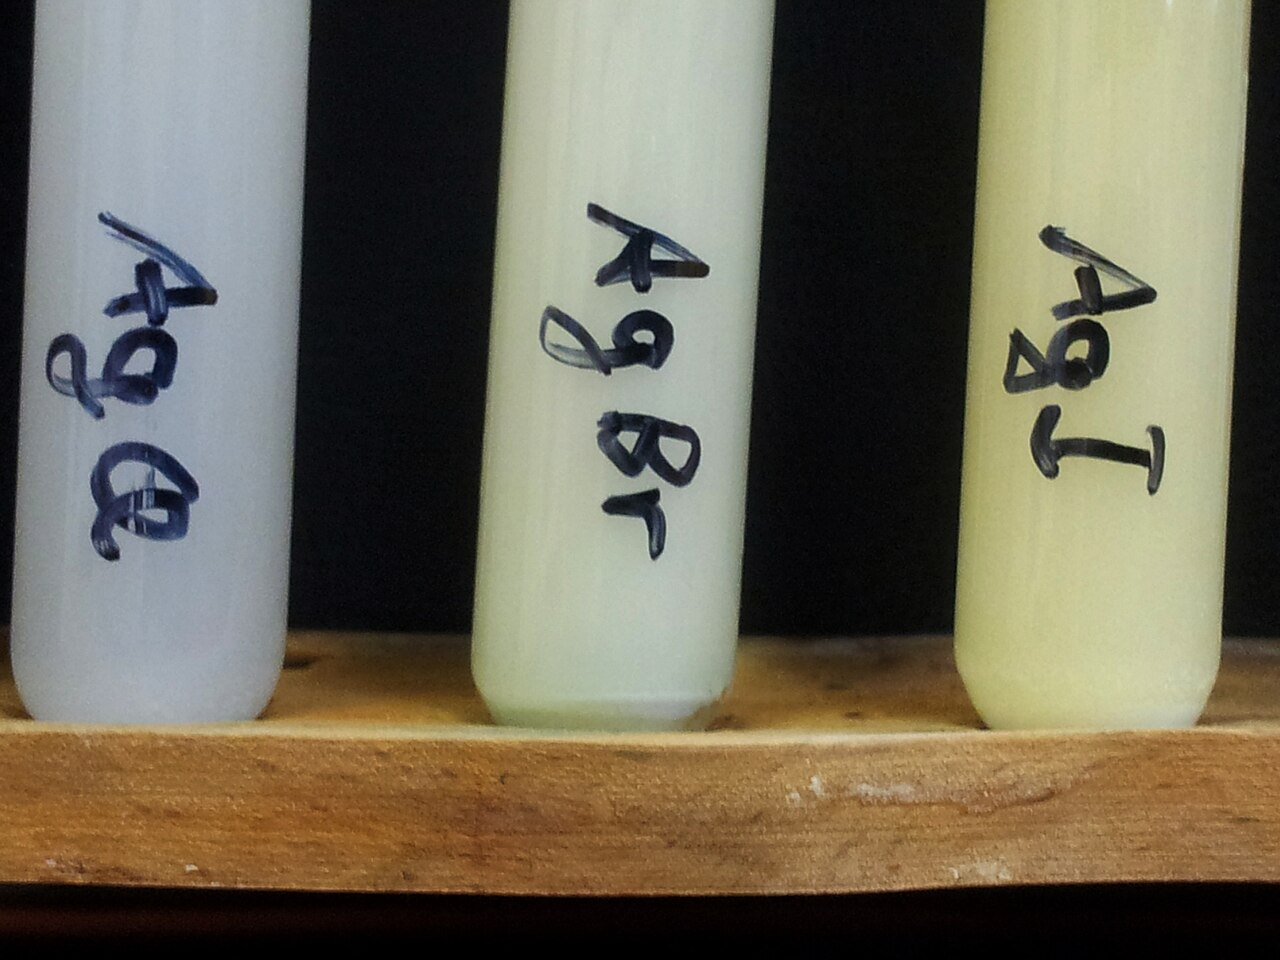
\includegraphics[width=0.6\linewidth]{images/book2/silver-halides.jpg}

{\small Endapan perak klorida (putih), perak bromida (krem), dan perak
iodida (kuning pucat). Foto Rrausch1974, CC BY-SA 3.0, Wikimedia
Commons.}
\end{omfigure}

\section{Kelarutan}

\begin{definition}[Kelarutan]\label{def:b1:precipitation:solubility}
\emph{Kelarutan}\index{kelarutan} $s$ sebuah padatan dalam suatu larutan
adalah jumlah padatan yang larut dalam satu liter larutan itu sampai
jenuh (dalam \unit{mol/L}); jika dikalikan dengan massa molar, diperoleh
kelarutan massa, dalam \unit{g/L}. Kelarutan bergantung pada suhu dan
pada komposisi larutan.
\end{definition}

\begin{proposition}[Kelarutan dari hasil kali kelarutan]\label{prop:b1:precipitation:s-of-ks}
Di dalam air murni, jika ion-ionnya tidak terlibat dalam reaksi lain,
\[
  \mathrm{MX}:\ s = \sqrt{K_s}, \qquad
  \mathrm{MX_2}\ \text{atau}\ \mathrm{M_2X}:\ s = \left(\frac{K_s}{4}\right)^{1/3},
  \qquad
  \mathrm{M}_a\mathrm{X}_b:\ s = \left(\frac{K_s}{a^a b^b}\right)^{1/(a+b)} .
\]
\end{proposition}

\begin{proof}
Jika $s$ mol padatan larut per liter, $[\mathrm{M}^{m+}] = as$ dan
$[\mathrm{X}^{x-}] = bs$, sehingga pada keadaan jenuh $K_s = (as)^a(bs)^b =
a^a b^b s^{a+b}$. Untuk MX, $a = b = 1$; untuk \ce{MX2}, $1^1 2^2 = 4$, dan
sama untuk \ce{M2X}.
\end{proof}

\begin{example}[Perak klorida dan perak kromat]\label{ex:b1:precipitation:agcl-ag2cro4}
Perak klorida: $s = 10^{-9.75/2} = \qty{1.3e-5}{mol/L}$, atau
\qty{1.9}{mg/L} dengan $M = \qty{143.4}{g/mol}$. Untuk perak kromat, \ce{Ag2CrO4}
($\mathrm{p}K_s = 11.95$): $s = (10^{-11.95}/4)^{1/3} =
\qty{6.6e-5}{mol/L}$. Kromat mempunyai $K_s$ yang lebih kecil, tetapi
lima kali lebih mudah larut. \omterm{def:b1:precipitation:solubility-product}{Hasil kali kelarutan} hanya dapat
dibandingkan langsung antara padatan-padatan dengan tipe rumus yang sama.
\end{example}

\begin{remark}
Rumus-rumus itu menganggap ion-ionnya bebas. Di dalam air murni ion
kromat adalah \omterm{def:b1:predominant-reaction:strong-acid}{basa lemah} dan ion perak tidak dikomplekskan oleh apa pun,
sehingga hasil untuk perak kromat hampir benar; untuk karbonat, sulfida,
atau hidroksida, sifat basa anionnya berpengaruh dan subbab berikutnya
diperlukan. Pada kekuatan ion yang tinggi, \omterm{def:b1:extent-q-and-k:activity}{aktivitas} juga menyimpang dari
konsentrasi, sebuah koreksi yang ditinggalkan untuk jilid Tahun~2.
\end{remark}

\section{Efek ion senama dan efek pH}

\begin{definition}[Efek ion senama]\label{def:b1:precipitation:common-ion}
\emph{Efek ion senama}\index{efek ion senama} adalah turunnya \omterm{def:b1:precipitation:solubility}{kelarutan}
sebuah padatan dalam larutan yang sudah mengandung salah satu ionnya.
\end{definition}

\begin{proposition}[Kelarutan dengan ion senama]\label{prop:b1:precipitation:common-ion}
Misalkan MX larut dalam larutan yang sudah mengandung $[\mathrm{X}^-] = c$,
dengan $c \gg \sqrt{K_s}$. Maka $s \approx K_s/c$, jauh lebih kecil
daripada di dalam air murni. Untuk \ce{MX2} dalam larutan yang
mengandung \ce{M^2+} pada $c$, $s \approx \frac12\sqrt{K_s/c}$.
\end{proposition}

\begin{proof}
Pada keadaan jenuh $[\mathrm{M}^+] = s$ dan $[\mathrm{X}^-] = c + s$,
sehingga $s(c + s) = K_s$. Jika $s \ll c$, $s = K_s/c$; anggapan ini
berlaku karena $K_s/c \ll c$ jika $c^2 \gg K_s$. Untuk \ce{MX2},
$[\ce{X-}] = 2s$ dan $[\mathrm{M}^{2+}] = c + s \approx c$, sehingga
$c\,(2s)^2 = K_s$.
\end{proof}

Perak klorida dalam natrium klorida \qty{0.10}{mol/L}: $s = 10^{-9.75}/0.10
= \qty{1.8e-9}{mol/L}$, tujuh ribu kali lebih sedikit daripada di dalam
air. Itulah sebabnya endapan dicuci dengan larutan encer yang mengandung
ion senama, bukan dengan air murni: endapan itu kehilangan lebih sedikit
dari dirinya.

Jika anion padatan itu sebuah basa, asam menariknya keluar dari
kesetimbangan pelarutan dan \omterm{def:b1:precipitation:solubility}{kelarutannya} naik. Untuk kalsium karbonat
dalam asam,
\[
  \ce{CaCO3(s) + H3O+ <=> Ca^2+ + HCO3- + H2O}, \qquad
  K = \frac{K_s}{K_{a2}} = 10^{-8.30 + 10.33} = 10^{2.03} ,
\]
reaksi yang disukai: cuka atau asam klorida melarutkan batu kapur, dan
karbon dioksida yang terbentuk melalui reaksi lanjut \ce{HCO3-} memberikan
buih yang sudah dikenal.
% ledger: dfg:HCO3-_ao (pKa2 of carbonic acid, ch. 10)

\begin{proposition}[Kelarutan hidroksida terhadap pH]\label{prop:b1:precipitation:hydroxide-ph}
Dalam larutan yang dibufer pada pH tertentu, konsentrasi \ce{M^{n+}} yang
berada dalam kesetimbangan dengan hidroksida \ce{M(OH)_n} mematuhi
\[
  \log[\mathrm{M}^{n+}] = -\mathrm{p}K_s + n\,(\mathrm{p}K_e - \mathrm{pH}) ,
\]
sebuah garis lurus dengan kemiringan $-n$ terhadap pH. Jika ion itu tidak
membentuk kompleks, inilah \omterm{def:b1:precipitation:solubility}{kelarutan} hidroksidanya.
\end{proposition}

\begin{proof}
$K_s = [\mathrm{M}^{n+}][\ce{OH-}]^n$ dan $[\ce{OH-}] = K_e/[\ce{H3O+}]$,
sehingga $\log[\mathrm{M}^{n+}] = \log K_s - n\log[\ce{OH-}] = -\mathrm{p}K_s -
n(\mathrm{pH} - \mathrm{p}K_e)$.
\end{proof}

Setiap satuan pH membagi \omterm{def:b1:precipitation:solubility}{kelarutan} besi(III) hidroksida dengan seribu dan
\omterm{def:b1:precipitation:solubility}{kelarutan} seng hidroksida dengan seratus. Hidroksida diendapkan, dan
dilarutkan kembali, dengan mengubah pH.

\begin{example}[Melarutkan kalsium karbonat dengan karbon dioksida]\label{ex:b1:precipitation:cave}
Air yang mengandung karbon dioksida terlarut melarutkan kalsit:
\[
  \ce{CaCO3(s) + CO2(aq) + H2O <=> Ca^2+ + 2HCO3-}, \qquad
  K = \frac{K_s K_{a1}}{K_{a2}} = 10^{-8.30 - 6.37 + 10.33} = 10^{-4.34} ,
\]
tetapan itu diperoleh dengan menjumlahkan pelarutan karbonat, keasaman
pertama karbon dioksida, dan kebalikan keasaman kedua. Makin banyak
karbon dioksida, makin banyak kalsium karbonat yang larut. Udara di dalam
tanah biasanya jauh lebih kaya karbon dioksida daripada udara gua; air
yang telah melintasi tanah dan mencapai langit-langit gua kehilangan
karbon dioksida, dan kalsit mengendap (\cref{exo:b1:precipitation:10}).
\end{example}

\section{Daerah keberadaan dan pengendapan selektif}\label{sec:b1:precipitation:domains}

\begin{definition}[Daerah keberadaan]\label{def:b1:precipitation:existence-domain}
Untuk sebuah padatan dan konsentrasi total $c$ salah satu ionnya,
\emph{daerah keberadaan}\index{daerah keberadaan} padatan itu adalah
rentang variabel (pX, pM, atau pH) tempat padatan itu ada pada
kesetimbangan. Batasnya adalah nilai ketika butir padatan pertama
muncul, yaitu ketika $Q_s = K_s$ dengan ion itu masih pada konsentrasi
$c$.
\end{definition}

\begin{method}[Menggambar diagram keberadaan]\label{met:b1:precipitation:existence-domain}
\begin{enumerate}
  \item Tetapkan konsentrasi total $c$ ion yang tidak berada pada sumbu
        (misalnya $[\ce{Ag+}]_{\mathrm{tot}} = c$ pada sumbu pCl).
  \item Tuliskan $K_s$ pada awal pengendapan, dengan ion itu masih pada
        $c$, lalu selesaikan untuk variabel pada sumbu.
  \item Padatan ada di sisi tempat ion yang lain pekat: pCl kecil (banyak
        klorida), pAg kecil, atau pH tinggi untuk hidroksida.
  \item Jangan menandai daerah untuk ion itu sendiri: ion itu ada di
        mana-mana, pada $c$ di luar daerah padatan dan di bawah $c$ di
        dalamnya.
\end{enumerate}
\end{method}

Untuk perak klorida dengan $c = [\ce{Ag+}]_{\mathrm{tot}} = 10^{-2}$:
pengendapan dimulai ketika $[\ce{Cl-}] = K_s/c = 10^{-7.75}$, sehingga
padatan itu ada untuk $\mathrm{pCl} < 7.75$. Untuk perak iodida batasnya
pada $\mathrm{pI} = 16.07 - 2 = 14.07$, seperti digambar di bawah.

\begin{omfigure}
\begin{tikzpicture}[font=\small, >={Stealth}, x=0.62cm]
  \fill[omDef!18] (0,0.12) rectangle (7.75,0.6);
  \draw[->, thick] (0,0) -- (17.2,0) node[right] {pCl atau pI};
  \foreach \x in {0,2,4,6,8,10,12,14,16}
    \draw (\x,0.08) -- (\x,-0.08) node[below] {\x};
  \draw[omDef, thick] (7.75,-0.5) -- (7.75,0.9);
  \node[omDef] at (3.9,0.36) {\ce{AgCl(s)} ada};
  \node[omDef, above] at (7.75,0.9) {7.75};
  \node[anchor=west] at (8.0,0.36) {tanpa padatan: \ce{Ag+} pada $10^{-2}$ mol/L};
  % AgI below
  \begin{scope}[yshift=-1.9cm]
  \fill[omProp!20] (0,0.12) rectangle (14.07,0.6);
  \draw[->, thick] (0,0) -- (17.2,0);
  \foreach \x in {0,2,4,6,8,10,12,14,16}
    \draw (\x,0.08) -- (\x,-0.08) node[below] {\x};
  \draw[omProp, thick] (14.07,-0.5) -- (14.07,0.9);
  \node[omProp] at (7.0,0.36) {\ce{AgI(s)} ada};
  \node[omProp, above] at (14.07,0.9) {14.07};
  \end{scope}
\end{tikzpicture}

{\small \omterm{def:b1:precipitation:existence-domain}{Daerah keberadaan} perak klorida (pada sumbu pCl, atas) dan perak
iodida (pada sumbu pI, bawah) untuk konsentrasi perak total
\qty{1.0e-2}{mol/L}. Iodida mengendapkan perak pada konsentrasi sejuta
kali lebih rendah daripada klorida.}
\end{omfigure}

\begin{method}[Pengendapan selektif]\label{met:b1:precipitation:selective}
Untuk memisahkan dua ion yang mengendap dengan pereaksi yang sama:
\begin{enumerate}
  \item hitunglah, untuk setiap ion pada konsentrasinya, konsentrasi
        pereaksi (atau pH) ketika padatannya mulai terbentuk; yang lebih
        rendah mengendap lebih dahulu;
  \item hitunglah konsentrasi ion pertama yang tersisa dalam larutan
        ketika ion kedua mulai mengendap;
  \item pemisahan itu dapat diterima jika konsentrasi tersebut merupakan
        bagian yang cukup kecil dari konsentrasi awal --- biasanya
        \qty{0.1}{\percent} --- dan penambahan pereaksi lalu dihentikan di
        antara kedua ambang.
\end{enumerate}
\end{method}

\begin{example}[Iodida dan klorida]\label{ex:b1:precipitation:i-cl}
Sebuah larutan mengandung ion iodida dan klorida, masing-masing
\qty{1.0e-2}{mol/L}; perak nitrat ditambahkan setetes demi setetes, tanpa
pengenceran. Perak iodida mulai terbentuk pada $[\ce{Ag+}] = 10^{-16.07 + 2} =
10^{-14.07}$, perak klorida pada $10^{-9.75 + 2} = 10^{-7.75}$: iodida
mengendap lebih dahulu. Ketika perak klorida muncul,
$[\ce{I-}] = 10^{-16.07}/10^{-7.75} = 10^{-8.32} = \qty{4.8e-9}{mol/L}$,
bagian $5 \times 10^{-7}$ dari iodida: pemisahannya sempurna.
\end{example}

Hidroksida dipisahkan dengan cara yang sama, dengan pH sebagai
variabelnya. Diagram di bawah memperlihatkan, untuk enam ion pada
\qty{0.010}{mol/L}, pH tempat hidroksida muncul dan pH tempat
\qty{99.9}{\percent} ion itu telah mengendap. Besi(III) dan aluminium
disingkirkan dalam air yang asam, seng dan besi(II) di sekitar netral,
magnesium di sekitar pH 10, dan kalsium hanya dalam air yang sangat basa.

\begin{omfigure}
\begin{tikzpicture}
\begin{axis}[
  width=0.82\linewidth, height=5.4cm, xmin=0, xmax=14, ymin=0.4, ymax=6.6,
  axis x line=bottom, axis y line=left, xlabel={pH},
  xtick={0,2,4,6,8,10,12,14}, ytick={1,2,3,4,5,6},
  yticklabels={\ce{Fe^3+}, \ce{Al^3+}, \ce{Zn^2+}, \ce{Fe^2+}, \ce{Mg^2+}, \ce{Ca^2+}},
  y dir=reverse, axis line style={-},
  tick label style={font=\small}, label style={font=\small}]
\addplot[draw=none, omDef!35,
  error bars/.cd, x dir=plus, x explicit,
  error bar style={line width=7pt, omDef!35}, error mark=none]
  table[x=start, y=row, x error expr=14-\thisrow{start}] {figdata/out/bachelor-1-solubility-ph-thresholds.dat};
\addplot[draw=none, omDef,
  error bars/.cd, x dir=plus, x explicit,
  error bar style={line width=7pt, omDef}, error mark=none]
  table[x=start, y=row, x error expr=\thisrow{end}-\thisrow{start}] {figdata/out/bachelor-1-solubility-ph-thresholds.dat};
\end{axis}
\end{tikzpicture}

{\small Pengendapan hidroksida dari larutan yang mengandung masing-masing
ion \qty{0.010}{mol/L}. Batang gelap membentang dari butir hidroksida
pertama sampai pH tempat \qty{99.9}{\percent} ion itu mengendap (selebar
satu satuan pH untuk ion trivalen, satu setengah untuk ion divalen);
batang terang adalah sisa \omterm{def:b1:precipitation:existence-domain}{daerah keberadaan} hidroksida itu. Pelarutan
kembali hidroksida seng dan aluminium yang amfoter pada pH tinggi
(\cref{sec:b1:precipitation:amphoteric}) tidak digambar.}
\end{omfigure}

\section{Hidroksida amfoter}\label{sec:b1:precipitation:amphoteric}

Tambahkan natrium hidroksida setetes demi setetes ke dalam larutan seng
sulfat: terbentuk endapan putih seng hidroksida, lalu, jika hidroksida
berlebih, endapan itu larut kembali. Aluminium hidroksida berperilaku
sama; besi(III) dan magnesium hidroksida tidak.

\begin{definition}[Hidroksida amfoter]\label{def:b1:precipitation:amphoteric-hydroxide}
Sebuah hidroksida disebut \emph{hidroksida amfoter}\index{hidroksida amfoter}
jika larut dalam asam, sebagai kation, dan juga dalam basa berlebih,
sebagai anion kompleks hidrokso:
\[
  \ce{Zn(OH)2(s) + 2H3O+ -> Zn^2+ + 4H2O}, \qquad
  \ce{Zn(OH)2(s) + 2OH- -> Zn(OH)4^2-} .
\]
\end{definition}

Anion kompleks \ce{Zn(OH)4^2-} (tetrahidroksozinkat) dicirikan oleh
tetapan pembentukannya $\beta_4 = [\ce{Zn(OH)4^2-}]/([\ce{Zn^2+}][\ce{OH-}]^4)
= 10^{14.45}$; kompleks dan tetapannya adalah pokok bahasan
\cref{ch:b1:complexation}.

\begin{proposition}[Kelarutan hidroksida amfoter]\label{prop:b1:precipitation:amphoteric}
Jika seng dalam larutan hanya terdapat sebagai \ce{Zn^2+} dan
\ce{Zn(OH)4^2-}, \omterm{def:b1:precipitation:solubility}{kelarutan} seng hidroksida adalah
\[
  s = [\ce{Zn^2+}] + [\ce{Zn(OH)4^2-}] = \frac{K_s}{[\ce{OH-}]^2} + K\,[\ce{OH-}]^2,
  \qquad K = \beta_4 K_s = 10^{-1.93} .
\]
Dalam $\log s$ terhadap pH, \omterm{def:b1:precipitation:solubility}{kelarutan} itu mengikuti garis berkemiringan
$-2$ pada pH rendah dan garis berkemiringan $+2$ pada pH tinggi.
\omterm{def:b1:precipitation:solubility}{Kelarutannya} paling kecil pada
$[\ce{OH-}]^4 = K_s/K = 1/\beta_4$, yaitu pada $\mathrm{pH} =
\mathrm{p}K_e - \frac14\log\beta_4$, dengan $s_{\min} = 2\sqrt{K_s K}$.
\end{proposition}

\begin{proof}
Pada keadaan jenuh berlaku $[\ce{Zn^2+}] = K_s/[\ce{OH-}]^2$, dan
$[\ce{Zn(OH)4^2-}] = \beta_4[\ce{Zn^2+}][\ce{OH-}]^4 = \beta_4 K_s
[\ce{OH-}]^2$. Dengan $w = [\ce{OH-}]^2$, $s(w) = K_s/w + Kw$ mempunyai turunan
$-K_s/w^2 + K$, yang nol pada $w = \sqrt{K_s/K}$, tempat $s = 2\sqrt{K_s K}$.
Pada pH rendah suku pertama dominan dan $\log s = \log K_s - 2\log[\ce{OH-}]$
(kemiringan $-2$ terhadap pH); pada pH tinggi suku kedua, $\log s = \log K + 2\log[\ce{OH-}]$
(kemiringan $+2$).
\end{proof}

Dengan nilai-nilai di atas, minimumnya terletak pada $\mathrm{pH} = 14.00 - 14.45/4
= 10.39$ dan $s_{\min} = 2 \times 10^{-(16.38 + 1.93)/2} =
\qty{1.4e-9}{mol/L}$
(gambar di bawah). Minimum yang sebenarnya jauh lebih tinggi: seng juga
membentuk \ce{ZnOH+}, \ce{Zn(OH)3-}, dan terutama \ce{Zn(OH)2(aq)} terlarut
yang tidak bermuatan, yang konsentrasinya dalam kesetimbangan dengan
padatan tidak bergantung pada pH. Perhitungan lengkap, dengan tabel yang
sama, menempatkan lantainya di dekat
$10^{-5.6}$~mol/L. Model dua spesies memberikan kemiringan dan urutan
ambang-ambangnya; di dekat minimum setiap spesies diperhitungkan.

\begin{omfigure}
\begin{tikzpicture}
\begin{axis}[name=zn,
  width=0.46\linewidth, height=5.6cm, xmin=6, xmax=14, ymin=-10, ymax=0,
  axis x line=bottom, axis y line=left, xlabel={pH}, ylabel={$\log s$},
  xtick={6,8,10,12,14}, ytick={-10,-8,-6,-4,-2,0},
  tick label style={font=\small}, label style={font=\small}]
\addplot[omProp, dashed, thick] table[x=pH, y=full] {figdata/out/bachelor-1-solubility-ph-zinc.dat};
\addplot[omDef, very thick] table[x=pH, y=model] {figdata/out/bachelor-1-solubility-ph-zinc.dat};
\node[font=\small, anchor=west] at (axis cs:7.0,-1.0) {\ce{Zn^2+}};
\node[font=\small, anchor=east] at (axis cs:13.8,-1.1) {\ce{Zn(OH)4^2-}};
\node[font=\small, omProp, anchor=south] at (axis cs:10.4,-5.5) {semua spesies};
\node[font=\small, anchor=north] at (axis cs:10.2,-0.4) {seng};
\end{axis}
\begin{axis}[at={(zn.east)}, anchor=west, xshift=1.8cm,
  width=0.46\linewidth, height=5.6cm, xmin=2, xmax=14, ymin=-10, ymax=0,
  axis x line=bottom, axis y line=left, xlabel={pH}, ylabel={$\log s$},
  xtick={2,4,6,8,10,12,14}, ytick={-10,-8,-6,-4,-2,0},
  tick label style={font=\small}, label style={font=\small}]
\addplot[omDef, very thick] table[x=pH, y=model] {figdata/out/bachelor-1-solubility-ph-aluminium.dat};
\node[font=\small, anchor=west] at (axis cs:3.4,-0.8) {\ce{Al^3+}};
\node[font=\small, anchor=east] at (axis cs:13.8,-0.6) {\ce{Al(OH)4-}};
\node[font=\small, anchor=north] at (axis cs:8.6,-0.4) {aluminium};
\end{axis}
\end{tikzpicture}

{\small \omterm{def:b1:precipitation:solubility}{Kelarutan} seng hidroksida (kiri) dan aluminium hidroksida, gibsit
(kanan), terhadap pH, model dua spesies (garis utuh): kemiringan $-2$ dan
$+2$ untuk seng, $-3$ dan $+1$ untuk aluminium. Untuk seng, kurva
putus-putus mencakup semua spesies hidrokso, dengan \ce{Zn(OH)2(aq)} yang
tidak bermuatan menetapkan sebuah lantai.}
\end{omfigure}

Untuk aluminium, hidroksidanya \ce{Al(OH)3} dan kompleksnya \ce{Al(OH)4-},
sehingga $\ce{Al(OH)3(s) + OH- <=> Al(OH)4-}$ dengan $K = \beta_4 K_s = 10^{33.52
- 34.75} = 10^{-1.23}$ dan kemiringan $-3$ dan $+1$. Perbedaan antara
aluminium dan besi(III) --- yang satu amfoter, yang lain tidak --- dipakai
dalam industri untuk memisahkan keduanya: natrium hidroksida panas
melarutkan aluminium dari bauksit dan meninggalkan oksida-oksida besi
(\cref{exo:b1:precipitation:12}).

\section{Latihan}

\begin{exercise}[$\star$]\label{exo:b1:precipitation:1}
Tuliskan persamaan pelarutan dan ungkapan $K_s$ untuk \ce{BaSO4},
\ce{CaF2}, \ce{Ag2CrO4}, dan \ce{Fe(OH)3}. Nyatakan $K_s$ dalam pangkat
sepuluh dari tabel pada \cref{sec:b1:precipitation:product}, serta
$\mathrm{p}K_s$ sebuah padatan dengan $K_s = \num{2.0e-13}$.
\end{exercise}

\begin{exercise}[$\star$]\label{exo:b1:precipitation:2}
Hitunglah \omterm{def:b1:precipitation:solubility}{kelarutan} perak bromida di dalam air murni dalam \unit{mol/L}
dan dalam \unit{mg/L} ($M = \qty{187.8}{g/mol}$).
\end{exercise}

\begin{exercise}[$\star$]\label{exo:b1:precipitation:3}
\qty{50}{mL} barium klorida \qty{2.0e-3}{mol/L} dicampur dengan
\qty{50}{mL} natrium sulfat \qty{2.0e-4}{mol/L}. Apakah barium sulfat
mengendap? Pertanyaan yang sama dengan natrium sulfat
\qty{2.0e-7}{mol/L}.
\end{exercise}

\begin{exercise}[$\star$]\label{exo:b1:precipitation:4}
Hitunglah \omterm{def:b1:precipitation:solubility}{kelarutan} barium sulfat di dalam air murni, lalu di dalam
larutan natrium sulfat \qty{0.010}{mol/L}. Dengan faktor berapakah
\omterm{def:b1:precipitation:solubility}{kelarutannya} berubah?
\end{exercise}

\begin{exercise}[$\star\star$]\label{exo:b1:precipitation:5}
Hitunglah \omterm{def:b1:precipitation:solubility}{kelarutan} kalsium fluorida di dalam air murni (\unit{mol/L} dan
\unit{mg/L}, $M = \qty{78.1}{g/mol}$), lalu di dalam larutan kalsium
klorida \qty{0.10}{mol/L}. Periksalah pendekatan yang dibuat.
\end{exercise}

\begin{exercise}[$\star\star$]\label{exo:b1:precipitation:6}
Sebuah larutan mengandung ion magnesium \qty{0.050}{mol/L}. Pada pH
berapakah magnesium hidroksida mulai mengendap? Pada pH berapakah
\qty{99}{\percent} magnesium telah mengendap? Gambarlah \omterm{def:b1:precipitation:existence-domain}{daerah keberadaan}
\ce{Mg(OH)2} pada sumbu pH.
\end{exercise}

\begin{exercise}[$\star\star$]\label{exo:b1:precipitation:7}
Sebuah larutan mengandung ion bromida dan klorida, masing-masing
\qty{1.0e-2}{mol/L}. Perak nitrat ditambahkan tanpa pengenceran. Endapan
manakah yang muncul lebih dahulu? Berapa bagian ion pertama yang masih
berada dalam larutan ketika padatan kedua muncul? Apakah pemisahannya
dapat diterima?
\end{exercise}

\begin{exercise}[$\star\star$]\label{exo:b1:precipitation:8}
Titrasi Mohr untuk klorida dengan ion perak memakai ion kromat sebagai
indikator: perak kromat yang merah hanya boleh muncul setelah hampir
semua klorida mengendap. Klorida \qty{0.050}{mol/L} dan kromat
\qty{5.0e-3}{mol/L}; pengenceran diabaikan. Hitunglah $[\ce{Ag+}]$ ketika
perak kromat mulai terbentuk, dan bagian klorida yang masih berada dalam
larutan pada saat itu.
\end{exercise}

\begin{exercise}[$\star\star$]\label{exo:b1:precipitation:9}
Kalsium karbonat dikocok dengan larutan yang pH-nya dijaga 8.30 oleh
sebuah penyangga, tempat hidrogenkarbonat merupakan spesies karbonat
yang jauh paling dominan. Tunjukkan bahwa
$[\ce{Ca^2+}][\ce{HCO3-}] = K_s\,10^{\mathrm{p}K_{a2} - \mathrm{pH}}$, lalu
hitunglah \omterm{def:b1:precipitation:solubility}{kelarutannya}, dengan anggapan bahwa semua karbonat yang larut
tetap sebagai \ce{HCO3-} ($\mathrm{p}K_{a2} = 10.33$).
\end{exercise}

\begin{exercise}[$\star\star\star$]\label{exo:b1:precipitation:10}
Gua batu kapur. \omterm{def:b1:precipitation:solubility}{Kelarutan} karbon dioksida mengikuti
\ce{CO2(g) <=> CO2(aq)} dengan $\log K_H = -1.47$ ($K_H =
[\ce{CO2(aq)}]/p(\ce{CO2})$, tekanan dalam bar).
\begin{enumerate}
  \item Gabungkan $K_H$ dengan tetapan pada
        \cref{ex:b1:precipitation:cave} untuk memperoleh tetapan
        \ce{CaCO3(s) + CO2(g) + H2O <=> Ca^2+ + 2HCO3-}.
  \item Tunjukkan bahwa \omterm{def:b1:precipitation:solubility}{kelarutan} kalsit adalah $s = (K'p/4)^{1/3}$, lalu
        hitunglah \omterm{def:b1:precipitation:solubility}{kelarutan} itu dalam air yang telah setimbang dengan
        udara tanah pada $p(\ce{CO2}) = \qty{0.010}{bar}$, lalu dengan
        udara luar, \qty{4.26e-4}{bar}. Nyatakan keduanya dalam
        \unit{mg/L} \ce{CaCO3} ($M = \qty{100.1}{g/mol}$).
  \item Jelaskan pertumbuhan sebuah stalaktit.
\end{enumerate}
\end{exercise}

\begin{exercise}[$\star\star\star$]\label{exo:b1:precipitation:11}
Sebuah larutan seng \qty{1.0e-2}{mol/L} dinaikkan pH-nya, dengan seng
hanya terdapat sebagai \ce{Zn^2+} dan \ce{Zn(OH)4^2-}.
\begin{enumerate}
  \item Di antara nilai pH berapakah seng hidroksida ada?
  \item Tentukan pH \omterm{def:b1:precipitation:solubility}{kelarutan} minimum dan \omterm{def:b1:precipitation:solubility}{kelarutan} minimumnya.
  \item Sketsalah $\log s$ terhadap pH dan berilah label kemiringannya.
\end{enumerate}
\end{exercise}

\begin{exercise}[$\star\star\star$]\label{exo:b1:precipitation:12}
Sebuah larutan mengandung ion aluminium dan besi(III), masing-masing
\qty{1.0e-3}{mol/L}. Natrium hidroksida ditambahkan berlebih.
\begin{enumerate}
  \item Di atas pH berapakah semua aluminium larut sebagai \ce{Al(OH)4-}?
  \item Berapa konsentrasi \ce{Fe^3+} pada saat itu? Simpulkan tentang
        pemisahannya.
  \item Jelaskan mengapa pemisahan itu akan gagal jika magnesium
        menggantikan aluminium.
\end{enumerate}
\end{exercise}

\section{Soal: Membersihkan Air Buangan Tambang}

\begin{problem}[{Soal akhir pekan --- ambang pengendapan tiga hidroksida,
kompleks hidrokso besi(III), pemulihan seng dan pelarutan kembalinya yang
amfoter, serta jendela pH untuk menyingkirkan besi(III) tanpa kehilangan
seng(II)}]
\label{pb:b1:precipitation:1}
Air yang mengalir dari sebuah tambang logam tua bersifat asam (pH 2.0)
dan mengandung besi(III) \qty{1.0e-3}{mol/L}, seng(II) \qty{5.0e-3}{mol/L},
dan magnesium \qty{2.0e-2}{mol/L}. Instalasi pengolahan menaikkan pH
setahap demi setahap untuk menyingkirkan besi sebagai lumpur limbah,
lalu untuk memulihkan seng sebagai hidroksidanya, sementara magnesium
yang tidak berbahaya dibiarkan di dalam air. Data pada
\qty{25}{\celsius}: $\mathrm{p}K_s$ \ce{Fe(OH)3} 38.55, \ce{Zn(OH)2}
16.38, \ce{Mg(OH)2} 11.25; $\log\beta_4(\ce{Zn(OH)4^2-}) = 14.45$;
$\log\beta_1(\ce{FeOH^2+}) = 11.82$; $\mathrm{p}K_e = 14.00$; massa molar
\ce{Fe(OH)3} \qty{106.8}{g/mol}, \ce{Zn(OH)2} \qty{99.4}{g/mol}.

\medskip
\noindent\textbf{Bagian I --- Hidroksida mana yang lebih dahulu?}
\begin{enumerate}
  \item Tuliskan kesetimbangan pelarutan ketiga hidroksida itu beserta
        $K_s$-nya.
  \item Jelaskan mengapa ketiga $\mathrm{p}K_s$ saja tidak menyatakan
        hidroksida mana yang mengendap lebih dahulu.
  \item Tunjukkan bahwa \ce{M(OH)_n} mulai mengendap dari larutan
        \ce{M^{n+}} pada $c$ pada $\mathrm{pH} = \mathrm{p}K_e -
        \frac1n(\mathrm{p}K_s + \log c)$.
  \item Hitunglah pH ini untuk besi(III).
  \item Hitunglah pH itu untuk seng.
  \item Hitunglah pH itu untuk magnesium.
  \item Tentukan urutan pengendapan seiring naiknya pH. Apakah ada yang
        mengendap dalam air buangan itu ketika keluar dari tambang?
\end{enumerate}

\medskip
\noindent\textbf{Bagian II --- Menyingkirkan besi: perkiraan pertama.}
\begin{enumerate}[resume]
  \item Instalasi itu menginginkan \qty{99.9}{\percent} besi keluar dari
        air. Konsentrasi besi terlarut berapakah yang diizinkan?
  \item Dengan mengabaikan kompleks apa pun, pada pH berapakah nilai itu
        tercapai?
  \item Tunjukkan bahwa, dalam \omterm{def:b1:precipitation:existence-domain}{daerah keberadaan} \ce{Fe(OH)3},
        $\log[\ce{Fe^3+}]$ turun 3 per satuan pH.
  \item Sampai pH berapakah seng tetap seluruhnya dalam larutan?
  \item Berikan perkiraan pertama jendela pH tempat besi disingkirkan
        sementara seng tetap tinggal.
\end{enumerate}

\medskip
\noindent\textbf{Bagian III --- Kompleks hidrokso besi(III).}
\begin{enumerate}[resume]
  \item Tuliskan pembentukan \ce{FeOH^2+} dari \ce{Fe^3+} dan \ce{OH-},
        beserta tetapannya.
  \item Gambarlah \omterm{def:b1:predominant-reaction:predominance}{diagram predominansi} \ce{Fe^3+} dan \ce{FeOH^2+}
        terhadap pH.
  \item Pada pH yang diperoleh pada pertanyaan 9, hitunglah
        $[\ce{FeOH^2+}]/[\ce{Fe^3+}]$. Apakah perkiraan pertama itu aman?
  \item Nyatakan besi terlarut total $[\ce{Fe^3+}] + [\ce{FeOH^2+}]$ yang
        berada dalam kesetimbangan dengan \ce{Fe(OH)3} sebagai fungsi pH.
  \item Tunjukkan bahwa, di daerah tempat \ce{FeOH^2+} predominan,
        logaritmanya turun 2 per satuan pH.
  \item Tentukan pH tempat besi terlarut total turun sampai nilai pada
        pertanyaan 8.
\end{enumerate}

\medskip
\noindent\textbf{Bagian IV --- Memulihkan seng.}
\begin{enumerate}[resume]
  \item Setelah lumpur besi disaring, pH dinaikkan lagi. Pada pH
        berapakah \qty{99}{\percent} seng telah mengendap? Apakah magnesium
        hidroksida terbentuk pada pH itu?
  \item Tuliskan reaksi seng hidroksida dengan ion hidroksida berlebih
        dan hitunglah tetapannya.
  \item Di atas pH berapakah semua seng akan kembali larut? Apa artinya
        bagi operator?
  \item Hitunglah massa lumpur besi(III) hidroksida yang disingkirkan per
        meter kubik air buangan.
  \item Hitunglah massa seng hidroksida yang dipulihkan per meter kubik
        pada pH pertanyaan 19.
  \item Mengapa besi harus disingkirkan sebelum seng, dan tidak
        keduanya sekaligus?
  \item Nyatakan jendela pH, sampai dua desimal, tempat besi(III)
        disingkirkan sampai \qty{99.9}{\percent} sementara seng(II) tetap
        seluruhnya dalam larutan.
\end{enumerate}
\end{problem}
